\documentclass{beamer}

\usepackage[british]{babel}
\usepackage{graphicx,hyperref,bsu,url}
\usepackage[export]{adjustbox}
\usepackage{subfigure}

% The title of the presentation:
%  - first a short version which is visible at the bottom of each slide;
%  - second the full title shown on the title slide;
\title[LDPC GPU Decoder]{
  Implementation of an LDPC Decoder on GPU of Mobile Devices}

% Optional: a subtitle to be dispalyed on the title slide
%\subtitle{Boise State University}%

% The author(s) of the presentation:
%  - again first a short version to be displayed at the bottom;
%  - next the full list of authors, which may include contact information;
\author[Roohollah Amiri]{
  Roohollah Amiri\\\medskip
  %{\small \url{roohollahamiri@u.boisestate.edu}} \\ 
 % {\small \url{https://github.com/ruhollahpython}}
 }

% The institute:
%  - to start the name of the university as displayed on the top of each slide
%    this can be adjusted such that you can also create a Dutch version
%  - next the institute information as displayed on the title slide
\institute[Boise State University]{
  Department of Electrical and Computer and Engineering \\
  Boise State University}

% Add a date and possibly the name of the event to the slides
%  - again first a short version to be shown at the bottom of each slide
%  - second the full date and event name for the title slide
\date[Parallel Computing 2016]{
  Parallel Computing\\
  May 2nd 2016}

\begin{document}

\begin{frame}
  \titlepage
\end{frame}

\begin{frame}
  \frametitle{Outline}

  \tableofcontents
\end{frame}

% Section titles are shown in at the top of the slides with the current section 
% highlighted. Note that the number of sections determines the size of the top 
% bar, and hence the university name and logo. If you do not add any sections 
% they will not be visible.
\section{LDPC Channel Coding}
%%%%
\begin{frame}
  \frametitle{LDPC Channel Coding}

\begin{figure}[h]
\begin{centering}
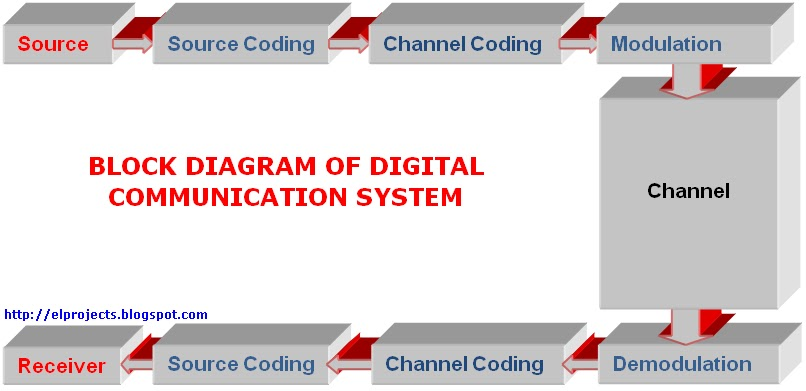
\includegraphics[scale=0.3]{img/Communication-System.png}
\caption[width=.3\textwidth]{Basic Building Blocks of a Communication System}
\end{centering}
\end{figure}

\end{frame}
%%%%
\begin{frame}
  \frametitle{LDPC Channel Coding}
  \textbf{Channel Coding}
    \begin{itemize}
    \item Channel Coding Adds Extra bits to each frame for error recognition at receiver
    \item Different Types as blocking, non-blocking, convolutional,...
  \end{itemize}
  \textbf{Low Density Parity Check Codes (LDPC)}
   \begin{itemize}
    \item can approach the Shannon limit to within 0.0045 dB
    \item applications including many communication standards such as IEEE 802.11n, 10 Gigabit Ethernet (IEEE 802.3an), Long Term Evolution (LTE) and DVB-S2
   \end{itemize}     
\end{frame}

%%%%
\begin{frame}
	\frametitle{LDPC Channel Coding}
	\textbf{LDPC Representation}

{\small
\begin{tabular}{p{3cm} l}
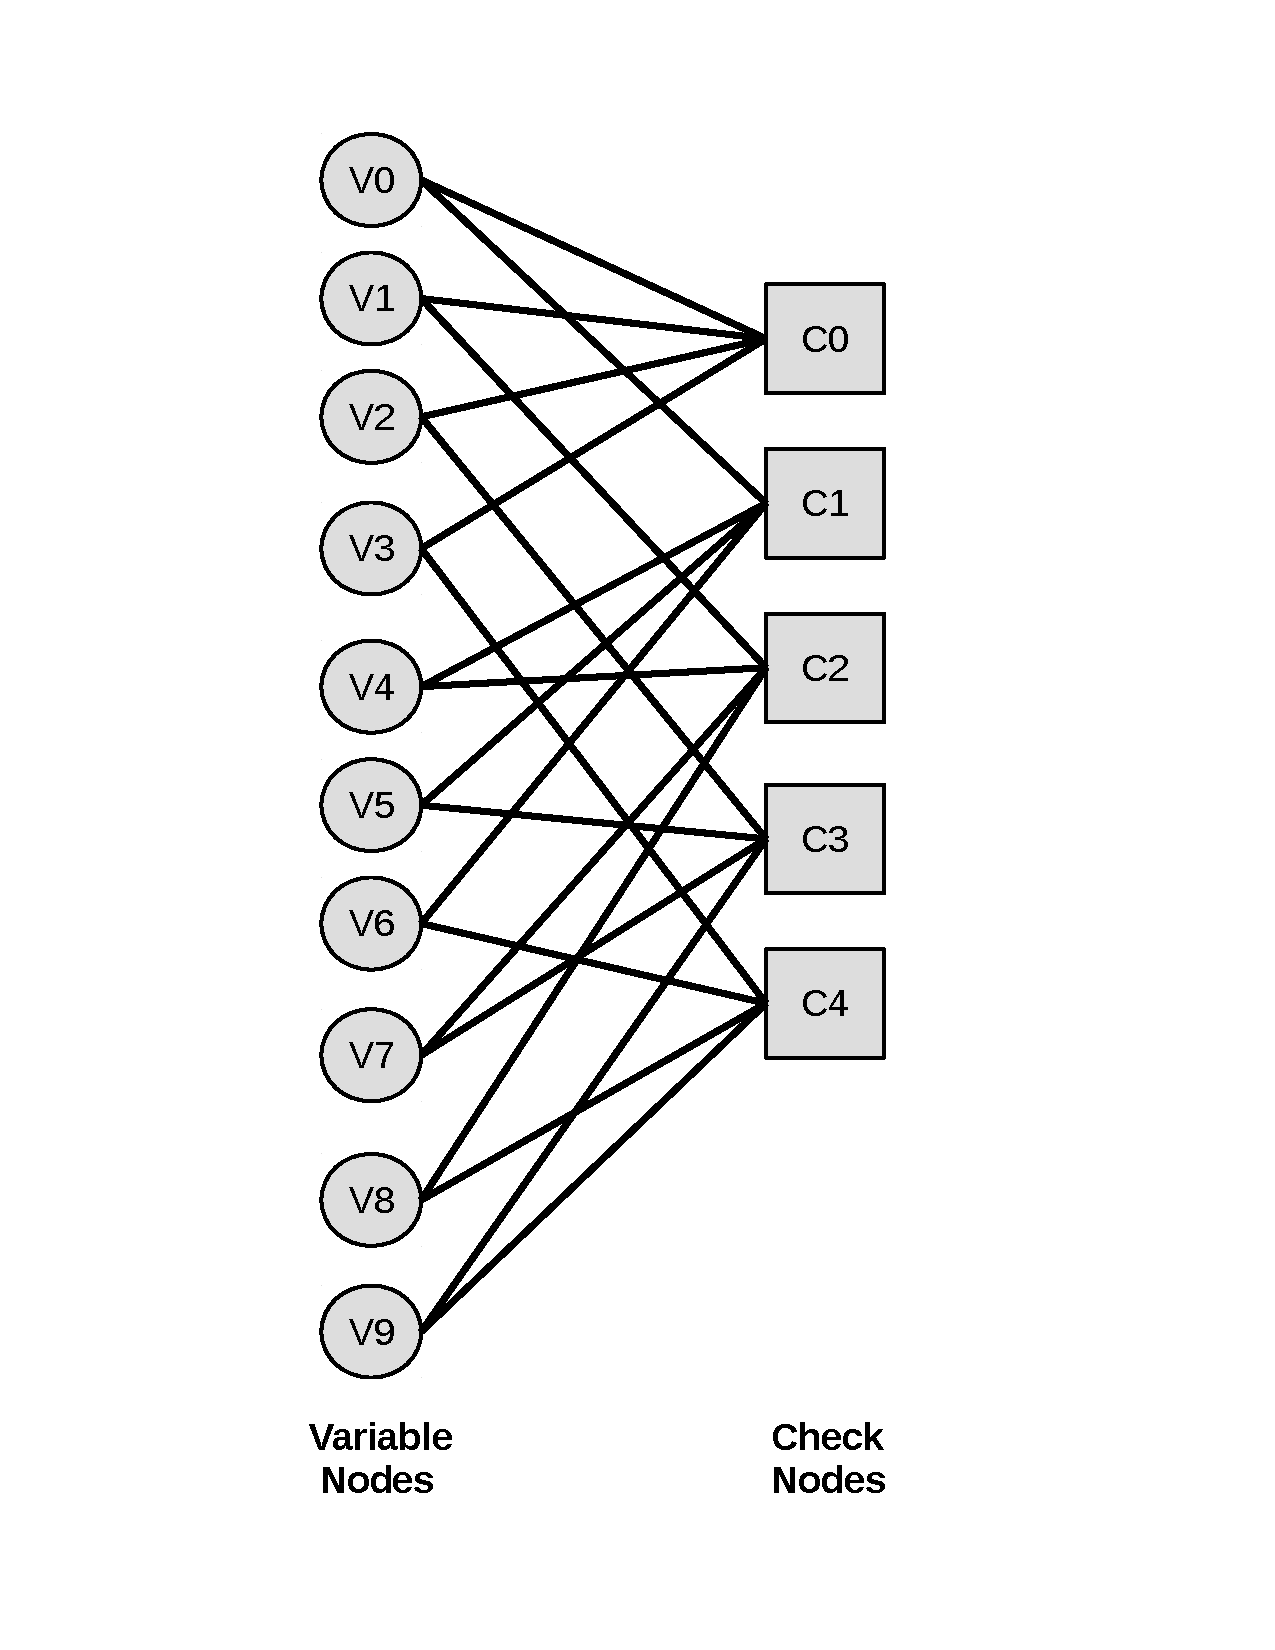
\includegraphics[keepaspectratio=true,width=.35\paperwidth,valign=c]{img/tanner.pdf}&
H=$\begin{bmatrix}
    1 & 1 & 1 & 1 & 0 &0 &0 &0 &0 &0 \\
    1 & 0 & 0 & 0 & 1 &1 &1 &0 &0 &0 \\
    0 & 1 & 0 & 0 & 1 &0 &0 &1 &1 &0 \\
    0 & 0 & 1 & 0 & 0 &1 &0 &1 &0 &1 \\
    0 & 0 & 0 & 1 & 0 &0 &1 &0 &1 &1 \\
  \end{bmatrix}$
  $, C\times H^{T}=0$ \end{tabular}}
\end{frame}

\section{Decoding Algorithm}

\begin{frame}
  \frametitle{Decoding Algorithm}
  \textbf{Belief Propagation}
  
  \begin{figure}[h]
\begin{centering}
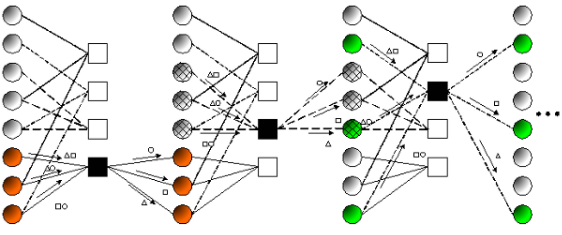
\includegraphics[scale=0.45]{img/decoding.png}
\caption[width=.3\textwidth]{Decoding of LDPC Codes}
\end{centering}
\end{figure}
  
\end{frame}

\begin{frame}
  \frametitle{Decoding Algorithm}
  \textbf{Implementation Challenges}
  
  \begin{itemize}
    \item The number of computations with respect to the number of memory access is low.
	\item The data reuse between consecutive computations is low.
	\item It requires a large set of irregular memory access due to the sparse nature of the H-matrix
  \end{itemize}
\end{frame}

%%%

\begin{frame}
  \frametitle{Decoding Algorithm}
	\textbf{Parallelism Levels in the Proposed Algorithm}
\begin{itemize}
  \item[$\bullet$ ] First parallelism level is located at the check node level. Two check node computations can be done in parallel if there is no data dependency.
\item[$\bullet$ ] Second parallelism level is located at the frame level (Complete execution of the Algorithm).
\end{itemize}

\begin{figure}[h]
\begin{centering}
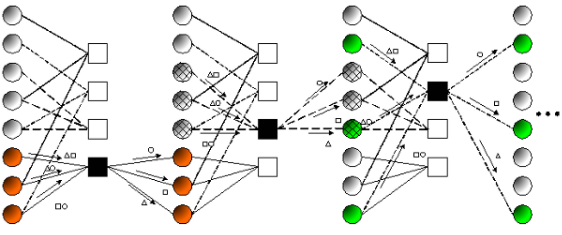
\includegraphics[scale=0.3]{img/decoding.png}
\end{centering}
\end{figure}
\end{frame}

\section{Implementation}

\begin{frame}
  \frametitle{Implementation}
	\textbf{Multi-Stream Parallelism}

{\small
\begin{tabular}{p{4cm} l}
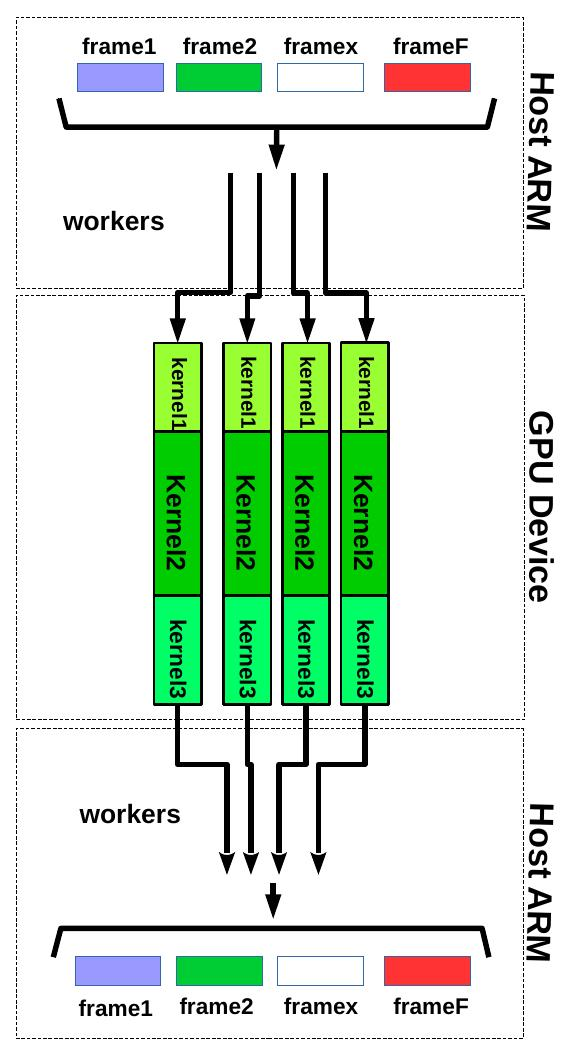
\includegraphics[keepaspectratio=true,width=.25\paperwidth,valign=c]{img/total_new.jpg}&
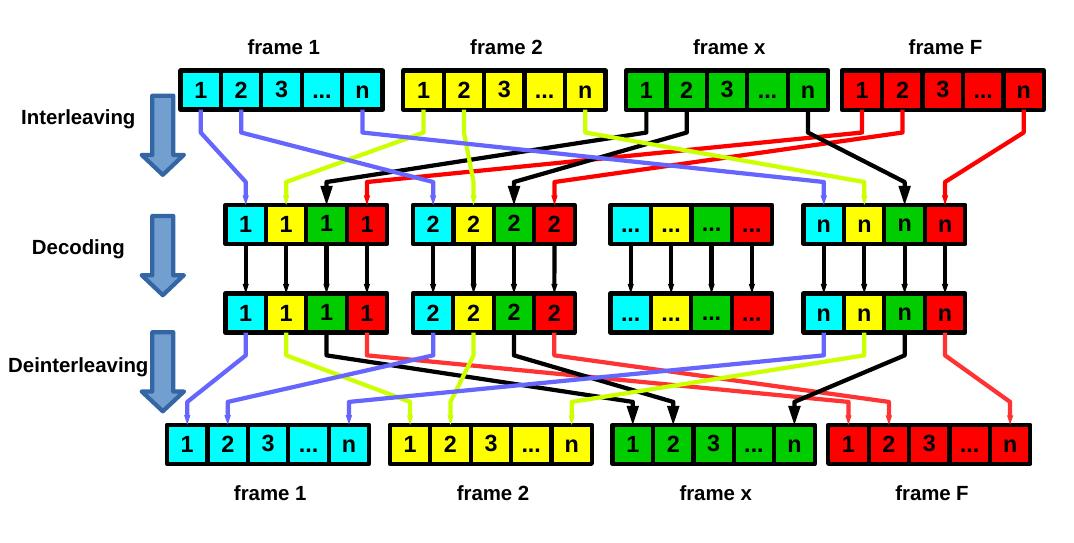
\includegraphics[keepaspectratio=true,width=.5\paperwidth,valign=c]{img/inter1.jpg}
   \end{tabular}}

\end{frame}

\section{Analysis of the work}

\begin{frame}
  \frametitle{Analysis of the work}
  \textbf{Target Architecture}
    \begin{figure}[h]
\begin{centering}
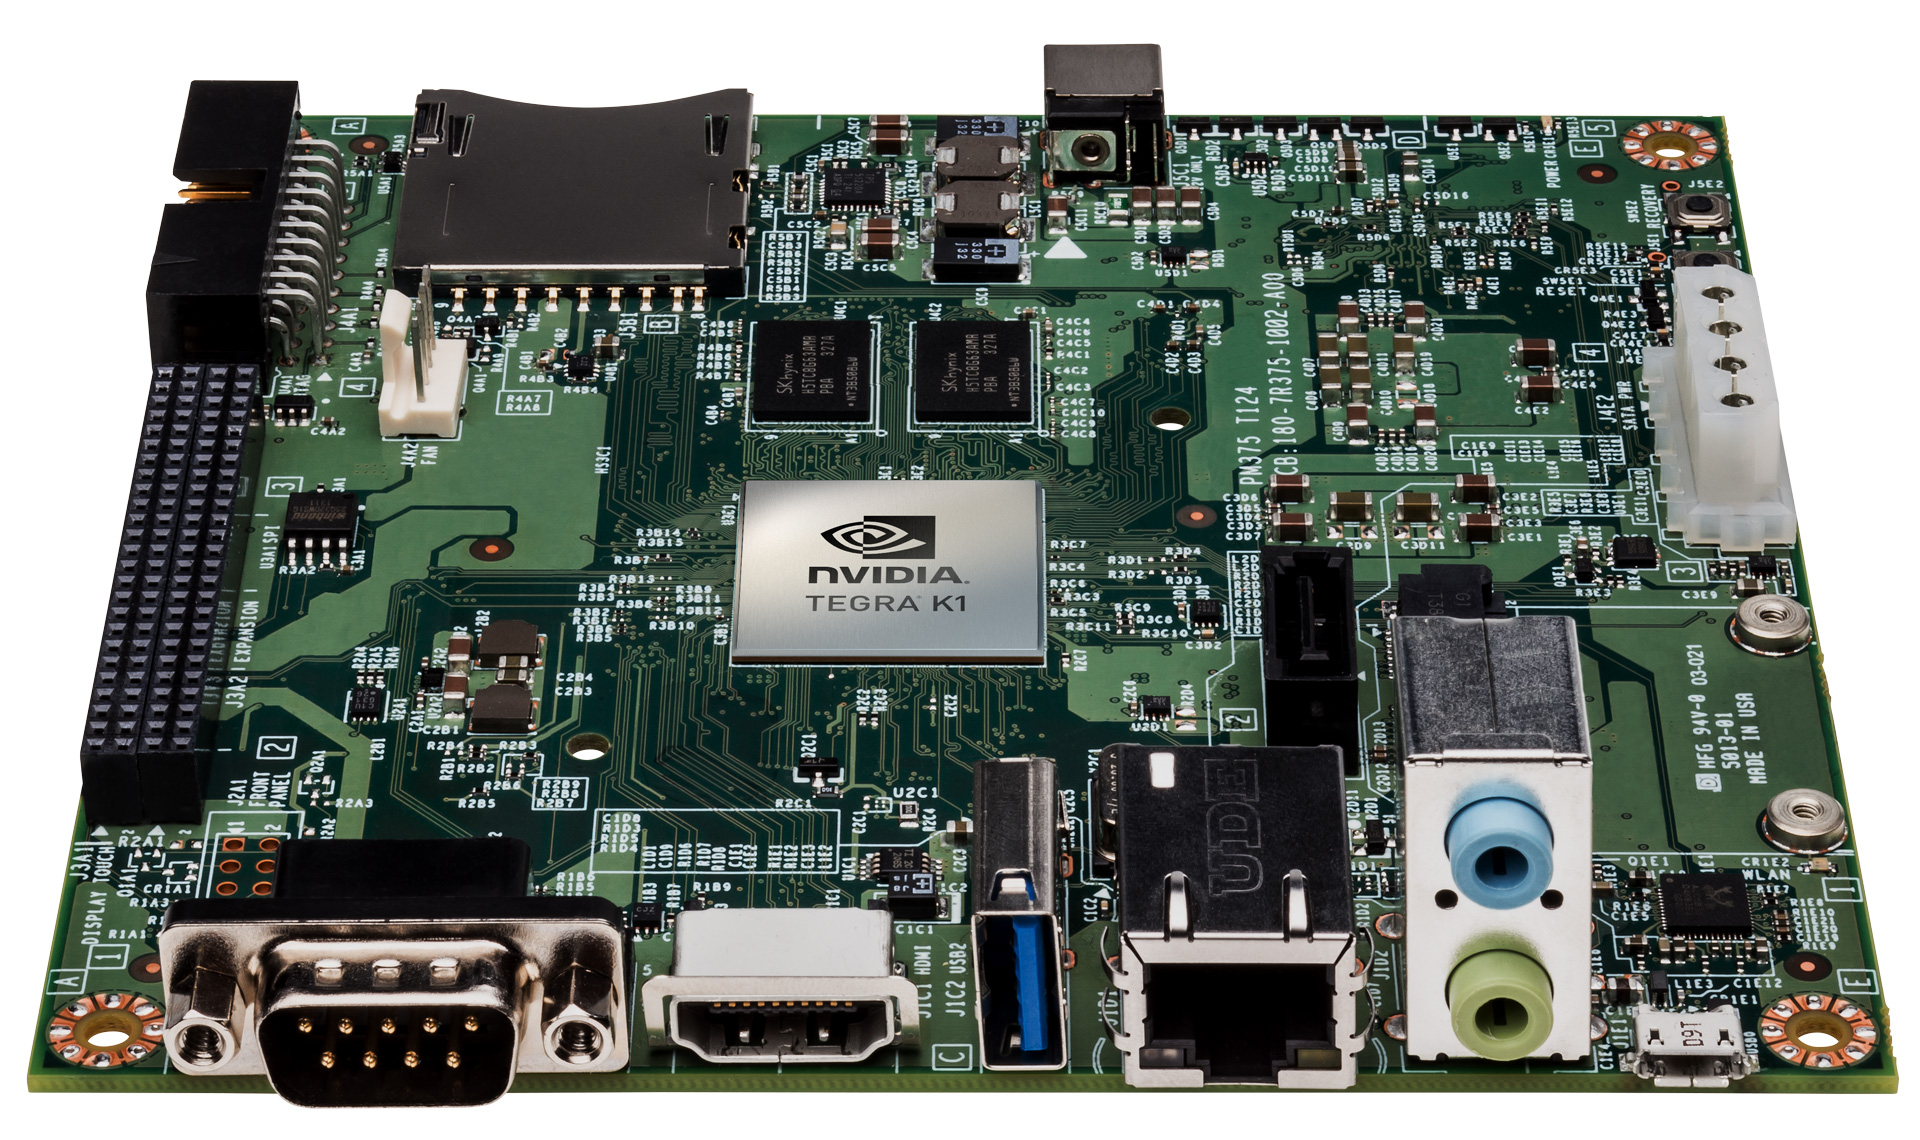
\includegraphics[scale=0.08]{img/Jetson_TK1.jpg}
\caption[width=.3\textwidth]{NVIDIA-Mobile Processor-GK20a, Kepler, CUDA 6.5}
\end{centering}
\end{figure}
  \end{frame}
%%%
\begin{frame}
  \frametitle{Analysis of the work}
  \textbf{Validating Results}
  
    \begin{figure}[h]
\begin{centering}
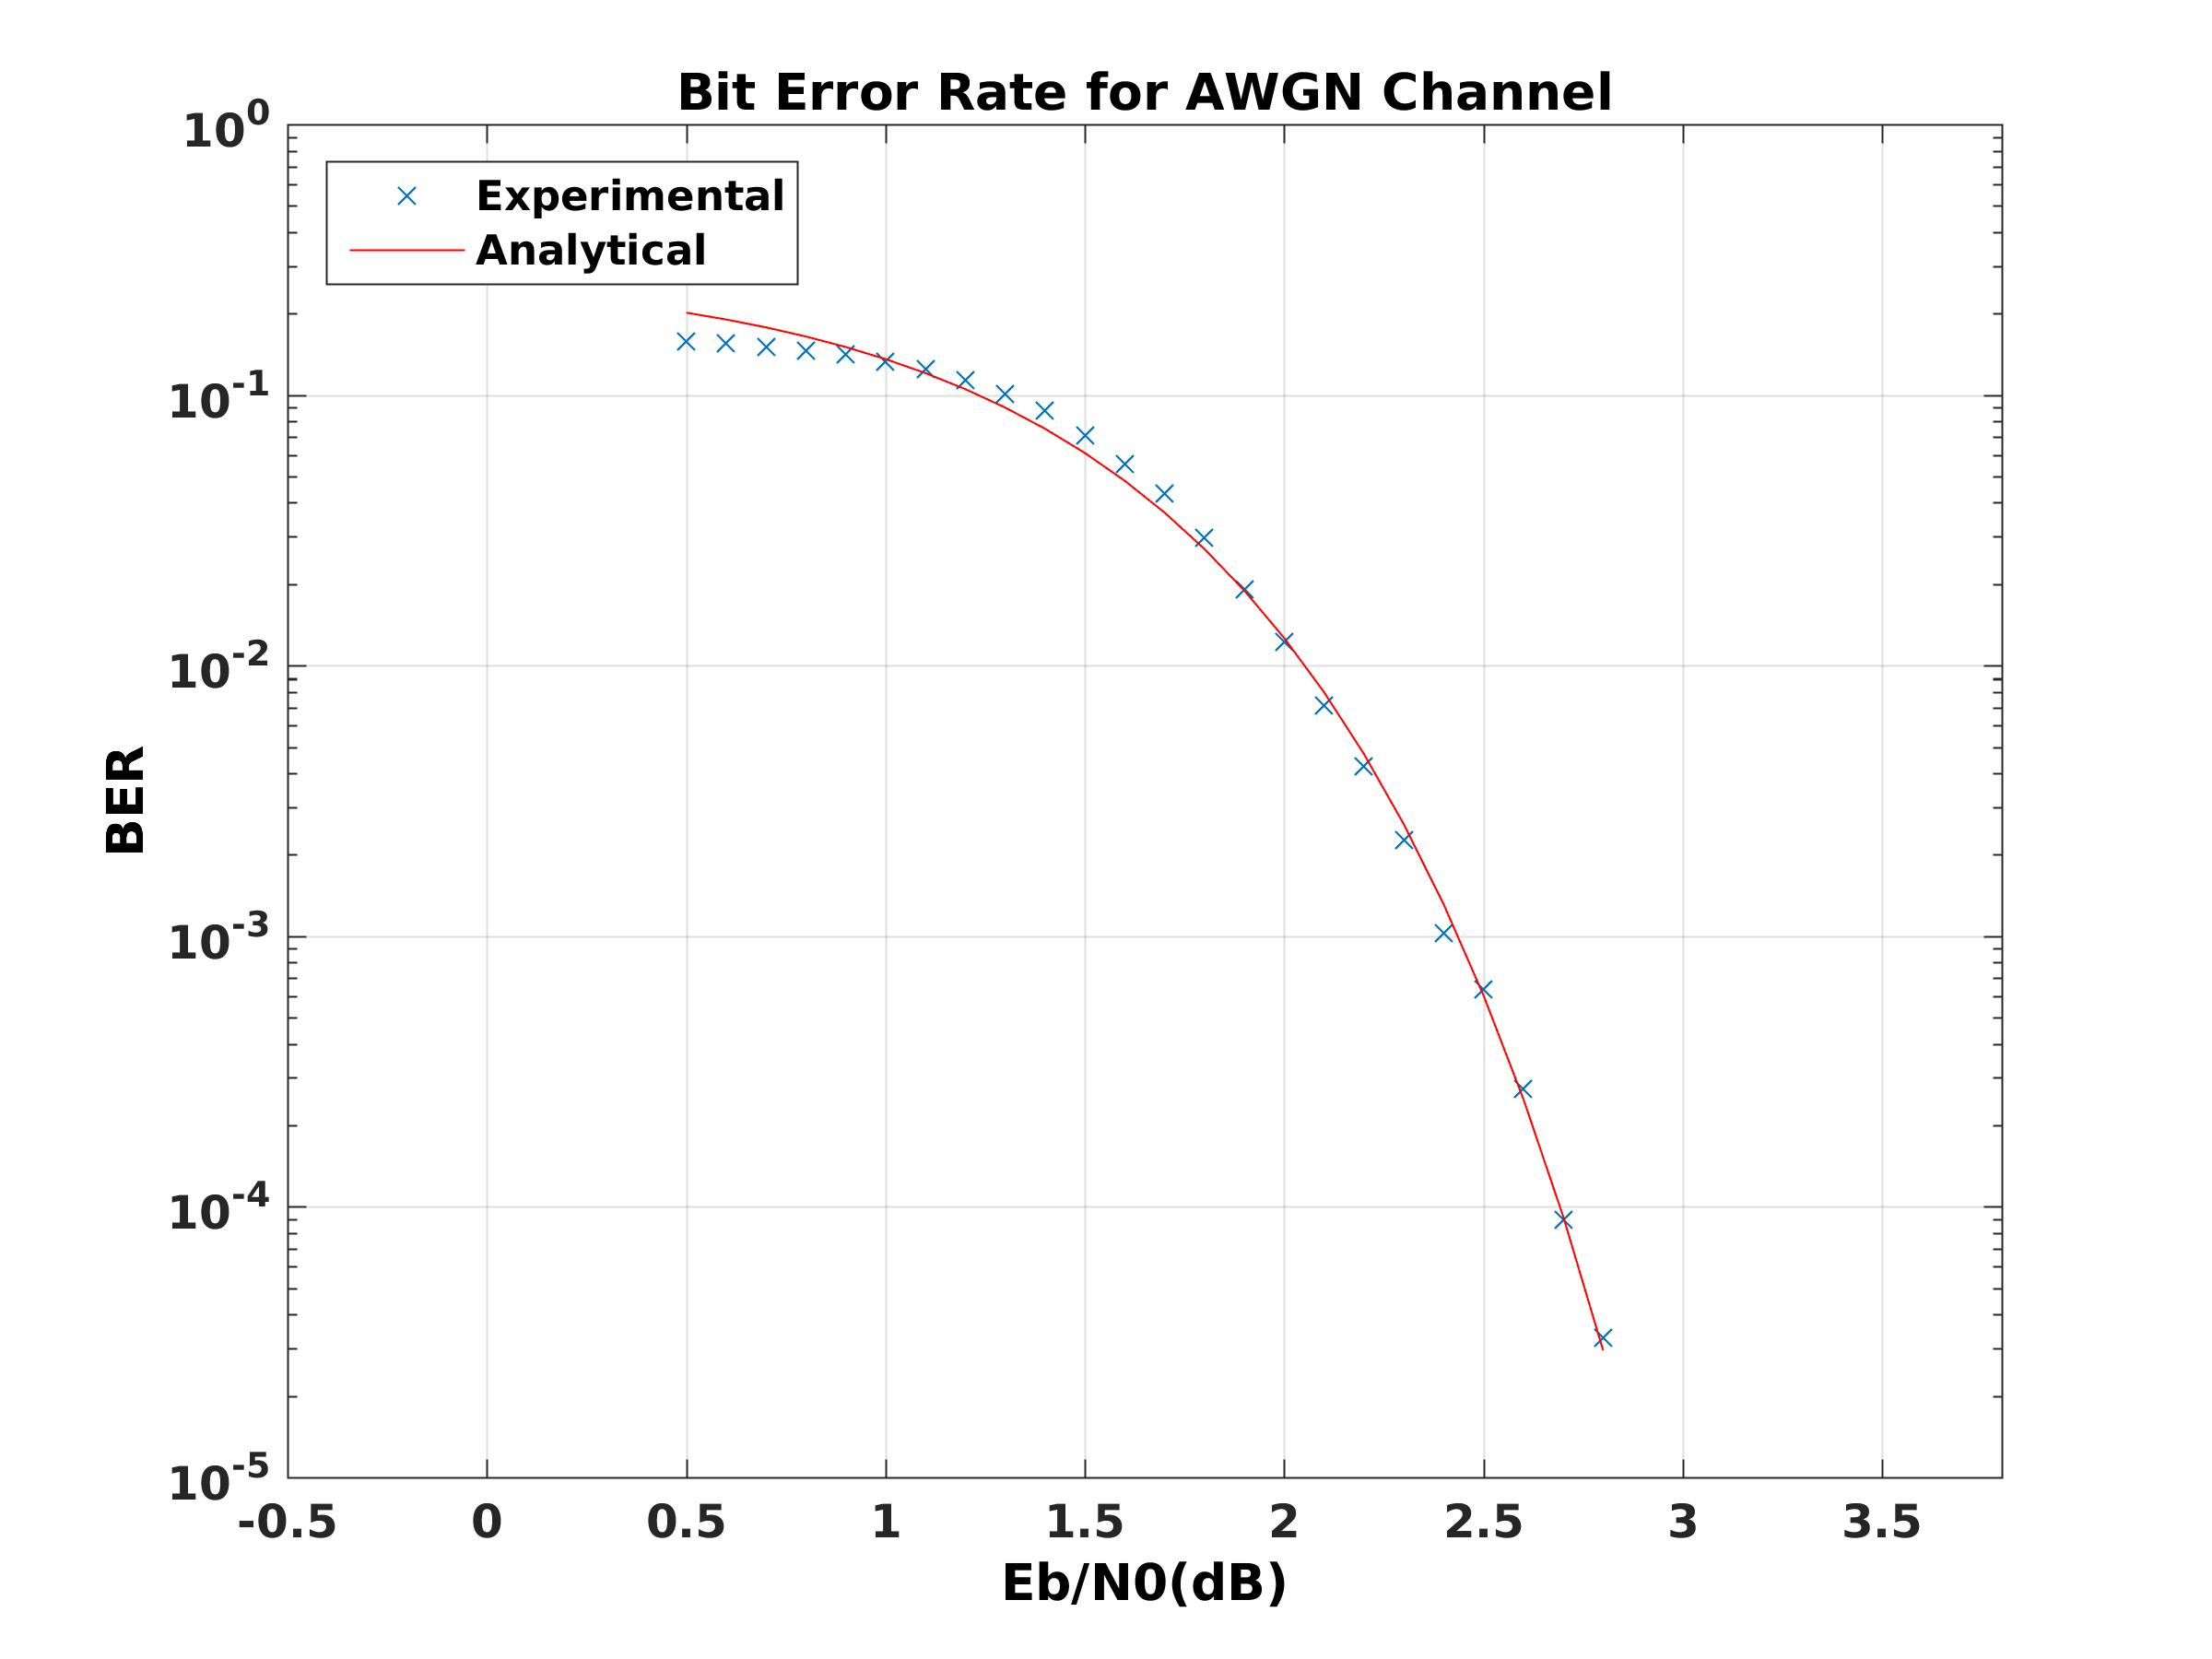
\includegraphics[scale=0.08]{img/BER.jpg}
\caption[width=.3\textwidth]{Bit Error Rate for AWGN Channel}
\end{centering}
\end{figure}
  \end{frame}
%%%%%
\begin{frame}
  \frametitle{Analysis of the work}
  \textbf{Throughput on Multiple Codes}
  \begin{figure}[h]
\begin{centering}
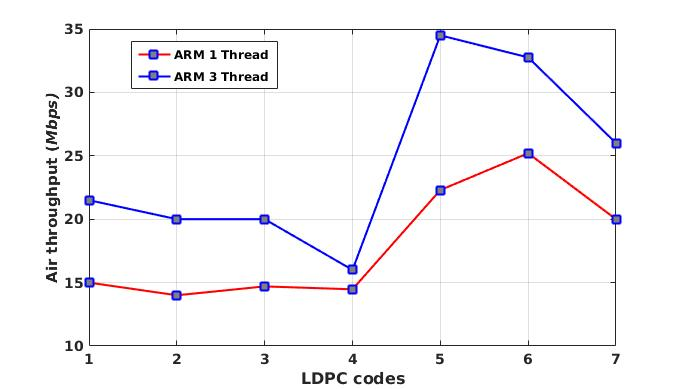
\includegraphics[scale=0.3]{img/air.jpg}
\caption[width=.5\textwidth]{Measured throughputs for 10 layered decoding iterations (1-7 LDPC codes: $576 \times 288, 1024 \times 512, 1200 \times 600, 1944 \times 722, 4000 \times 2000, 8000 \times 4000, 9972 \times 4086$)}
\end{centering}
\end{figure}
  
\end{frame}
%%%
\begin{frame}
  \frametitle{Analysis of the work}
  \textbf{Throughput on Multiple Devices}

  \begin{figure}
    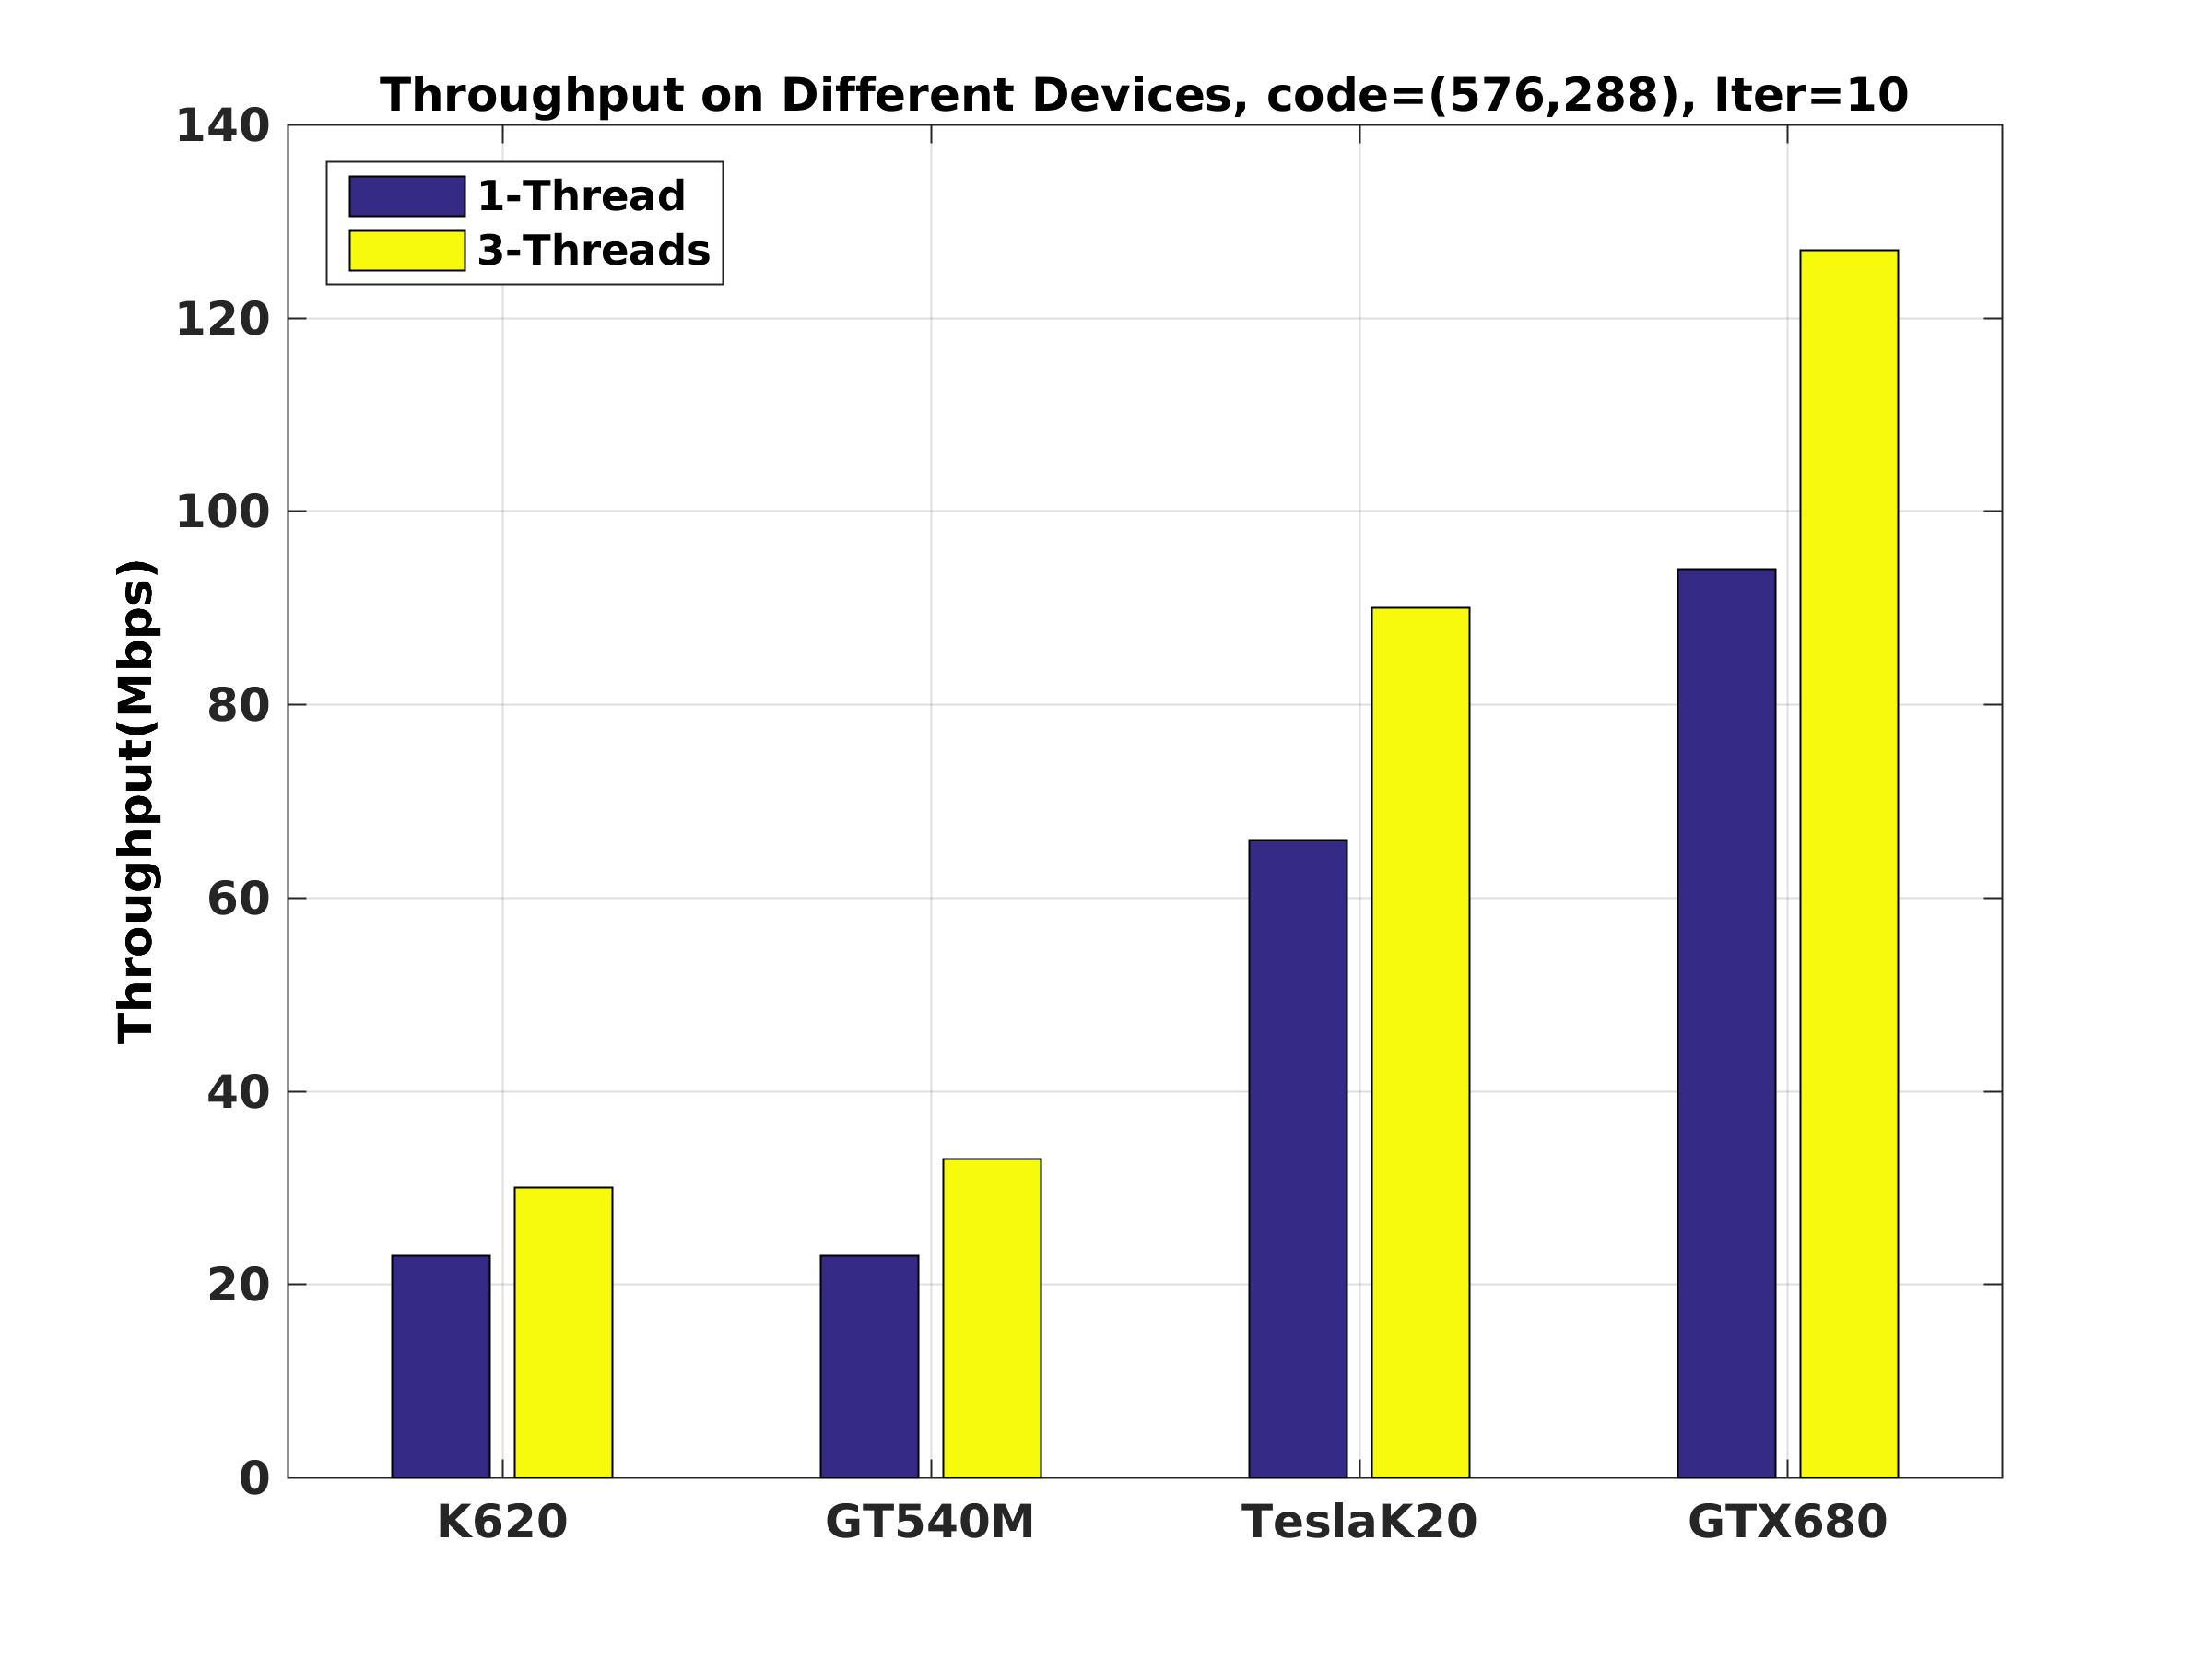
\includegraphics[width=0.65\textwidth]{img/c_576_10.jpg}
    \caption{code=(576,288)}
  \end{figure}
  %
%  \begin{subfigure}[b]{0.6\textwidth}
%    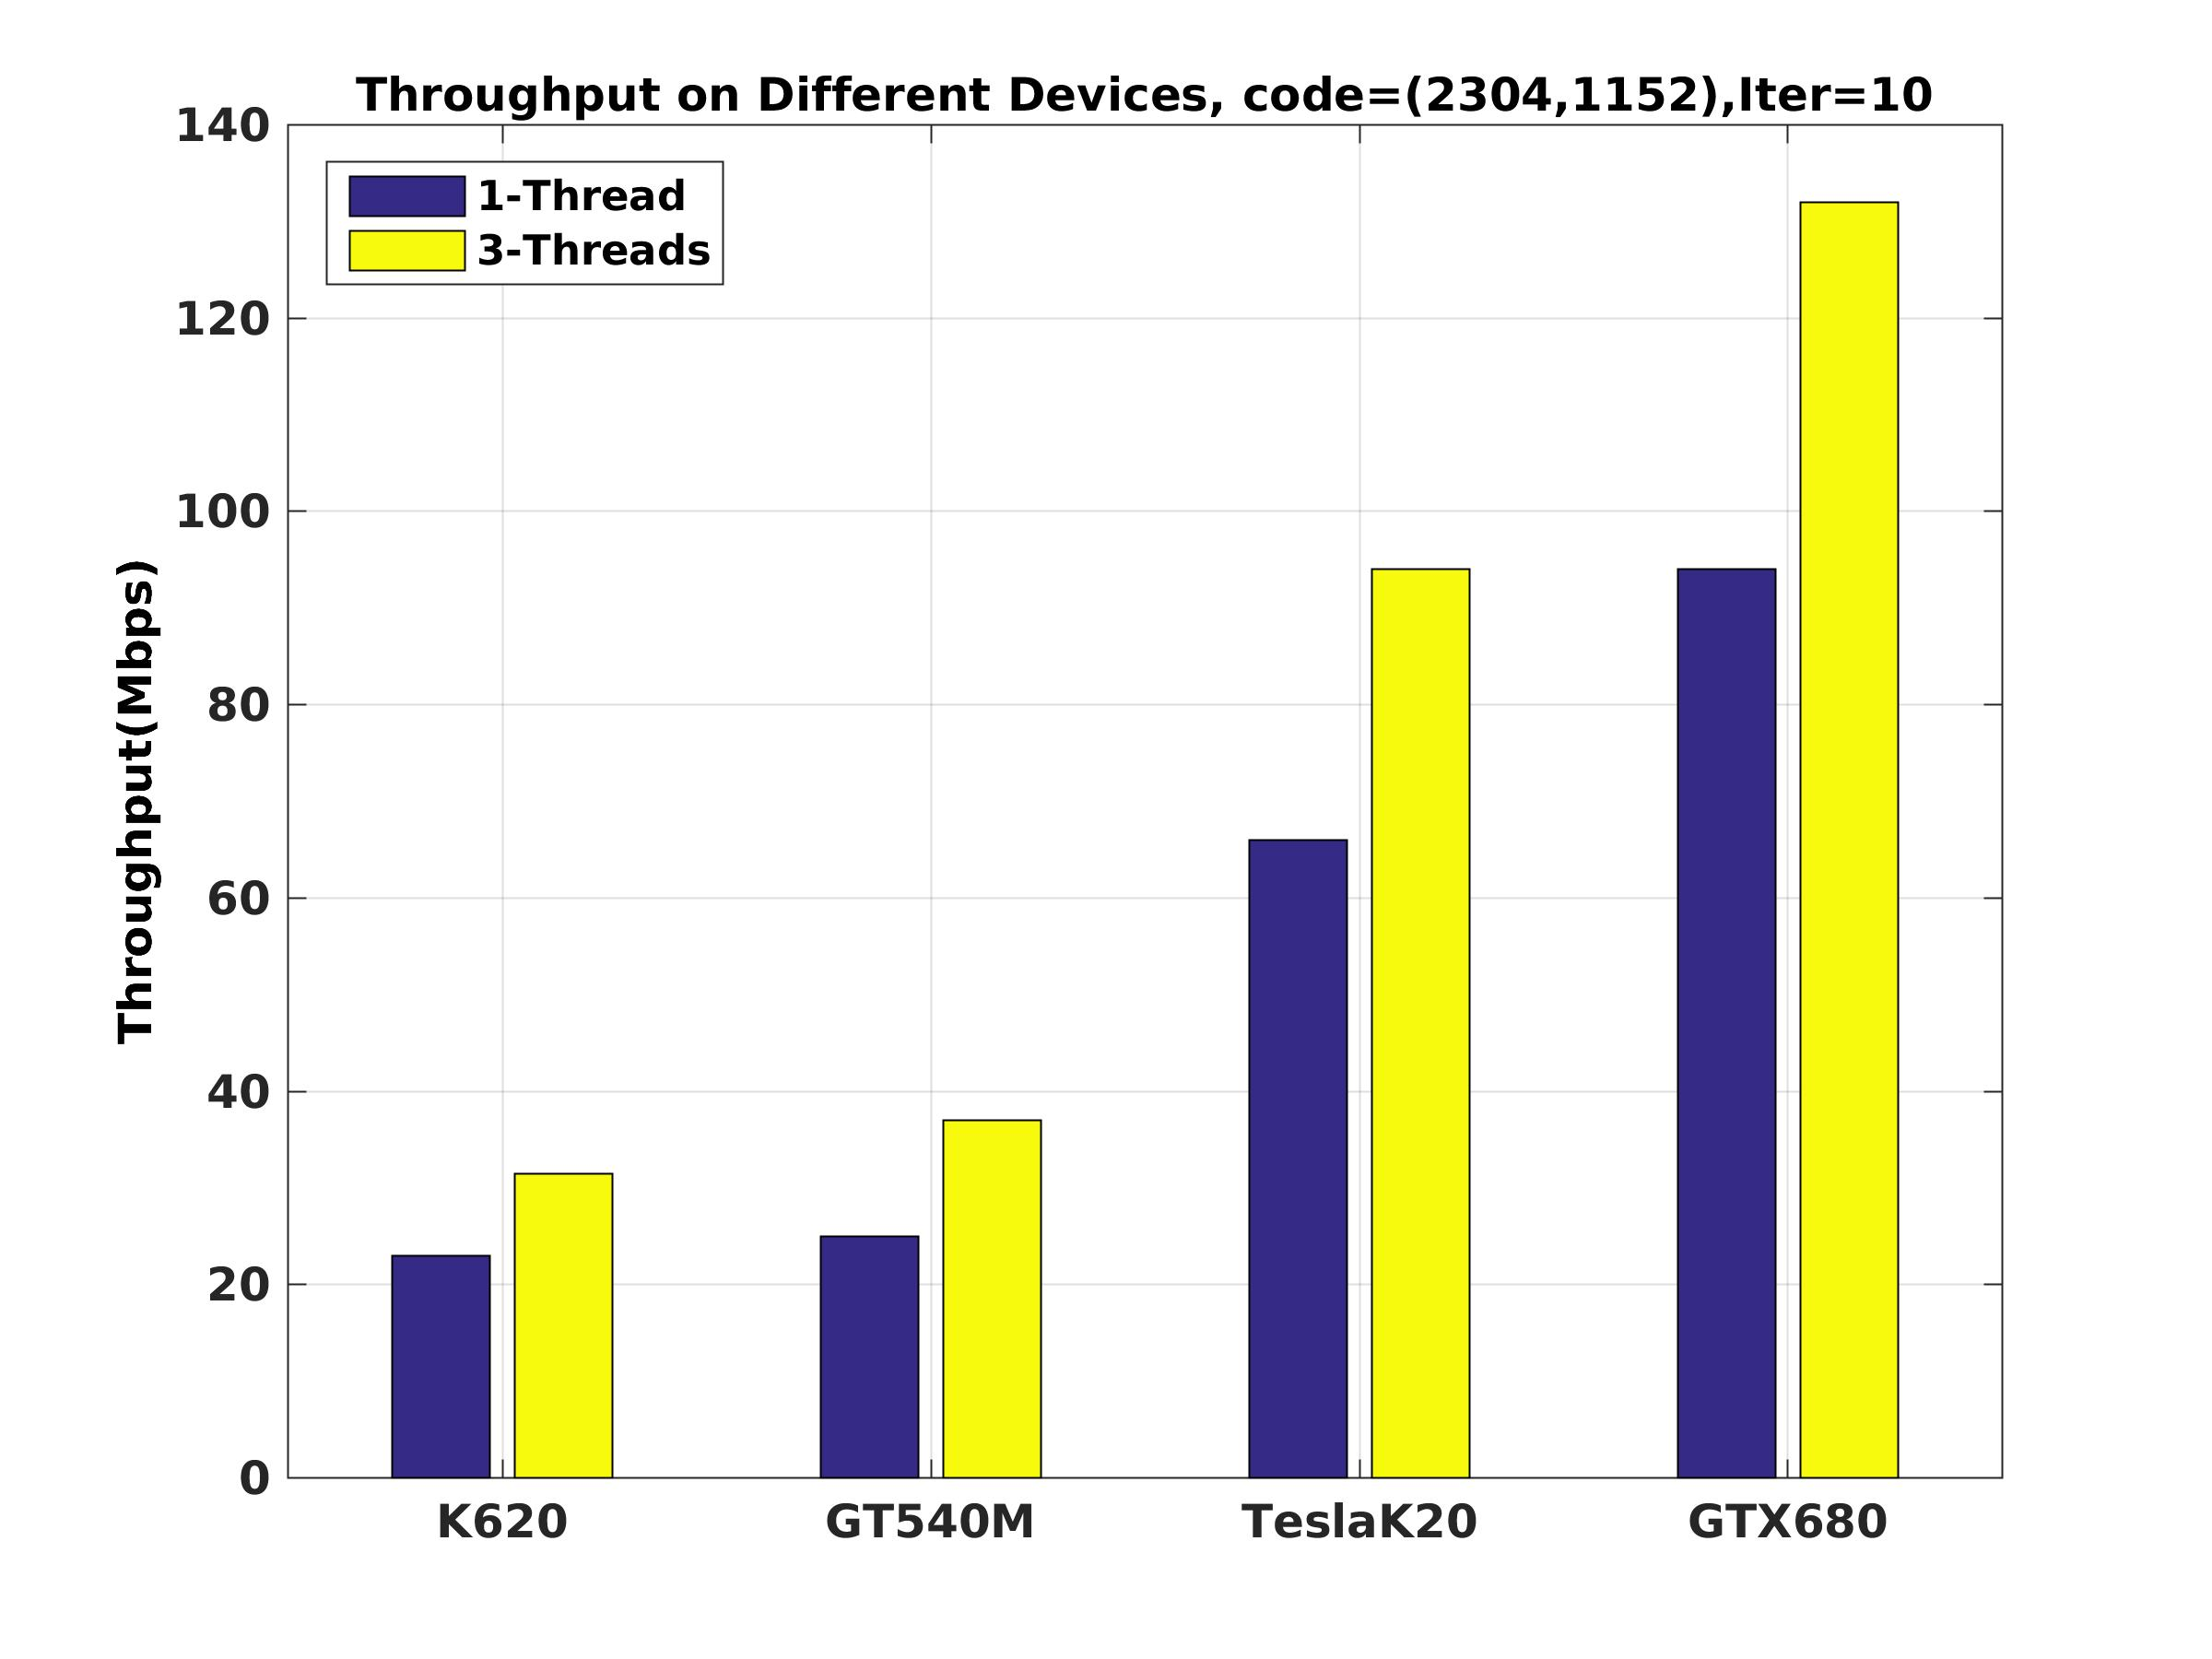
\includegraphics[width=\textwidth]{img/c_2304_10.jpg}
%    \caption{code=(2304,1152)}
%  \end{subfigure}
%  \\
%    \begin{subfigure}[b]{0.7\textwidth}
%    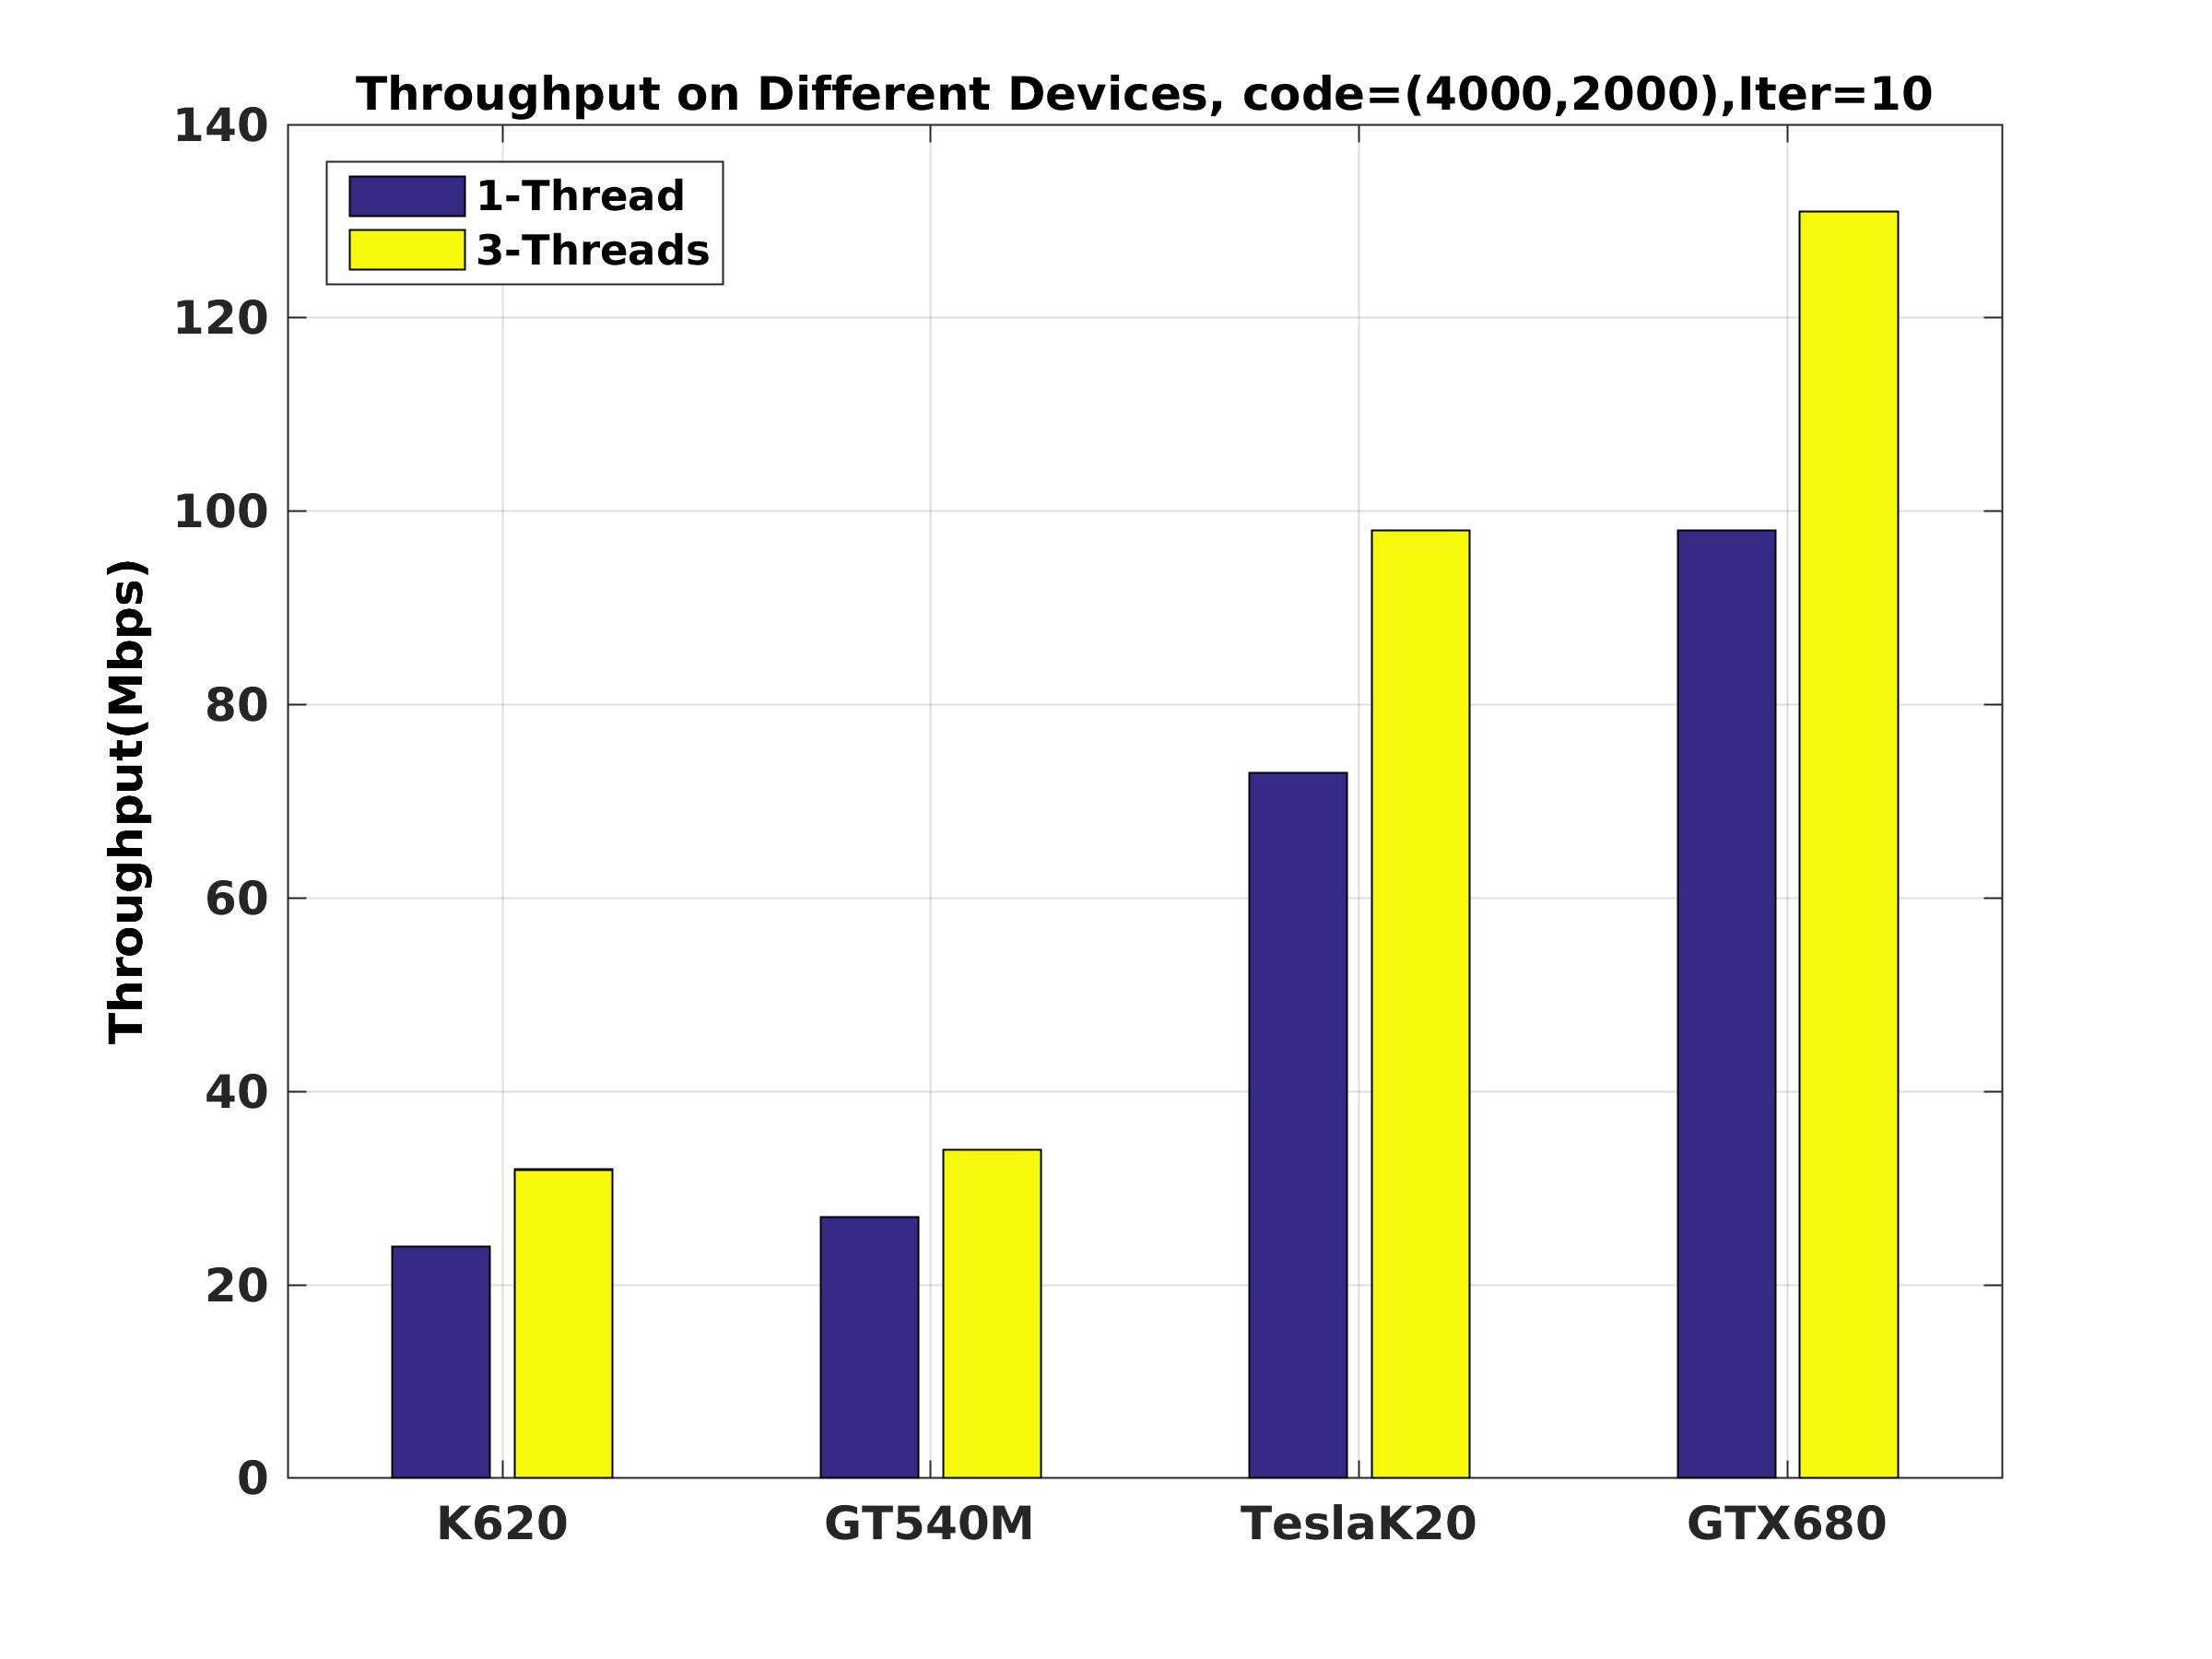
\includegraphics[width=\textwidth]{img/c_4k_10.jpg}
%    \caption{code=(4000,2000)}
%  \end{subfigure}
%  \caption{10 Iteration experiment}\label{fig:10iter}
%\end{figure}
  
  \end{frame}
  
  %%%
  \begin{frame}
  \frametitle{Analysis of the work}
  \textbf{Throughput on Multiple Devices}
    \begin{figure}
    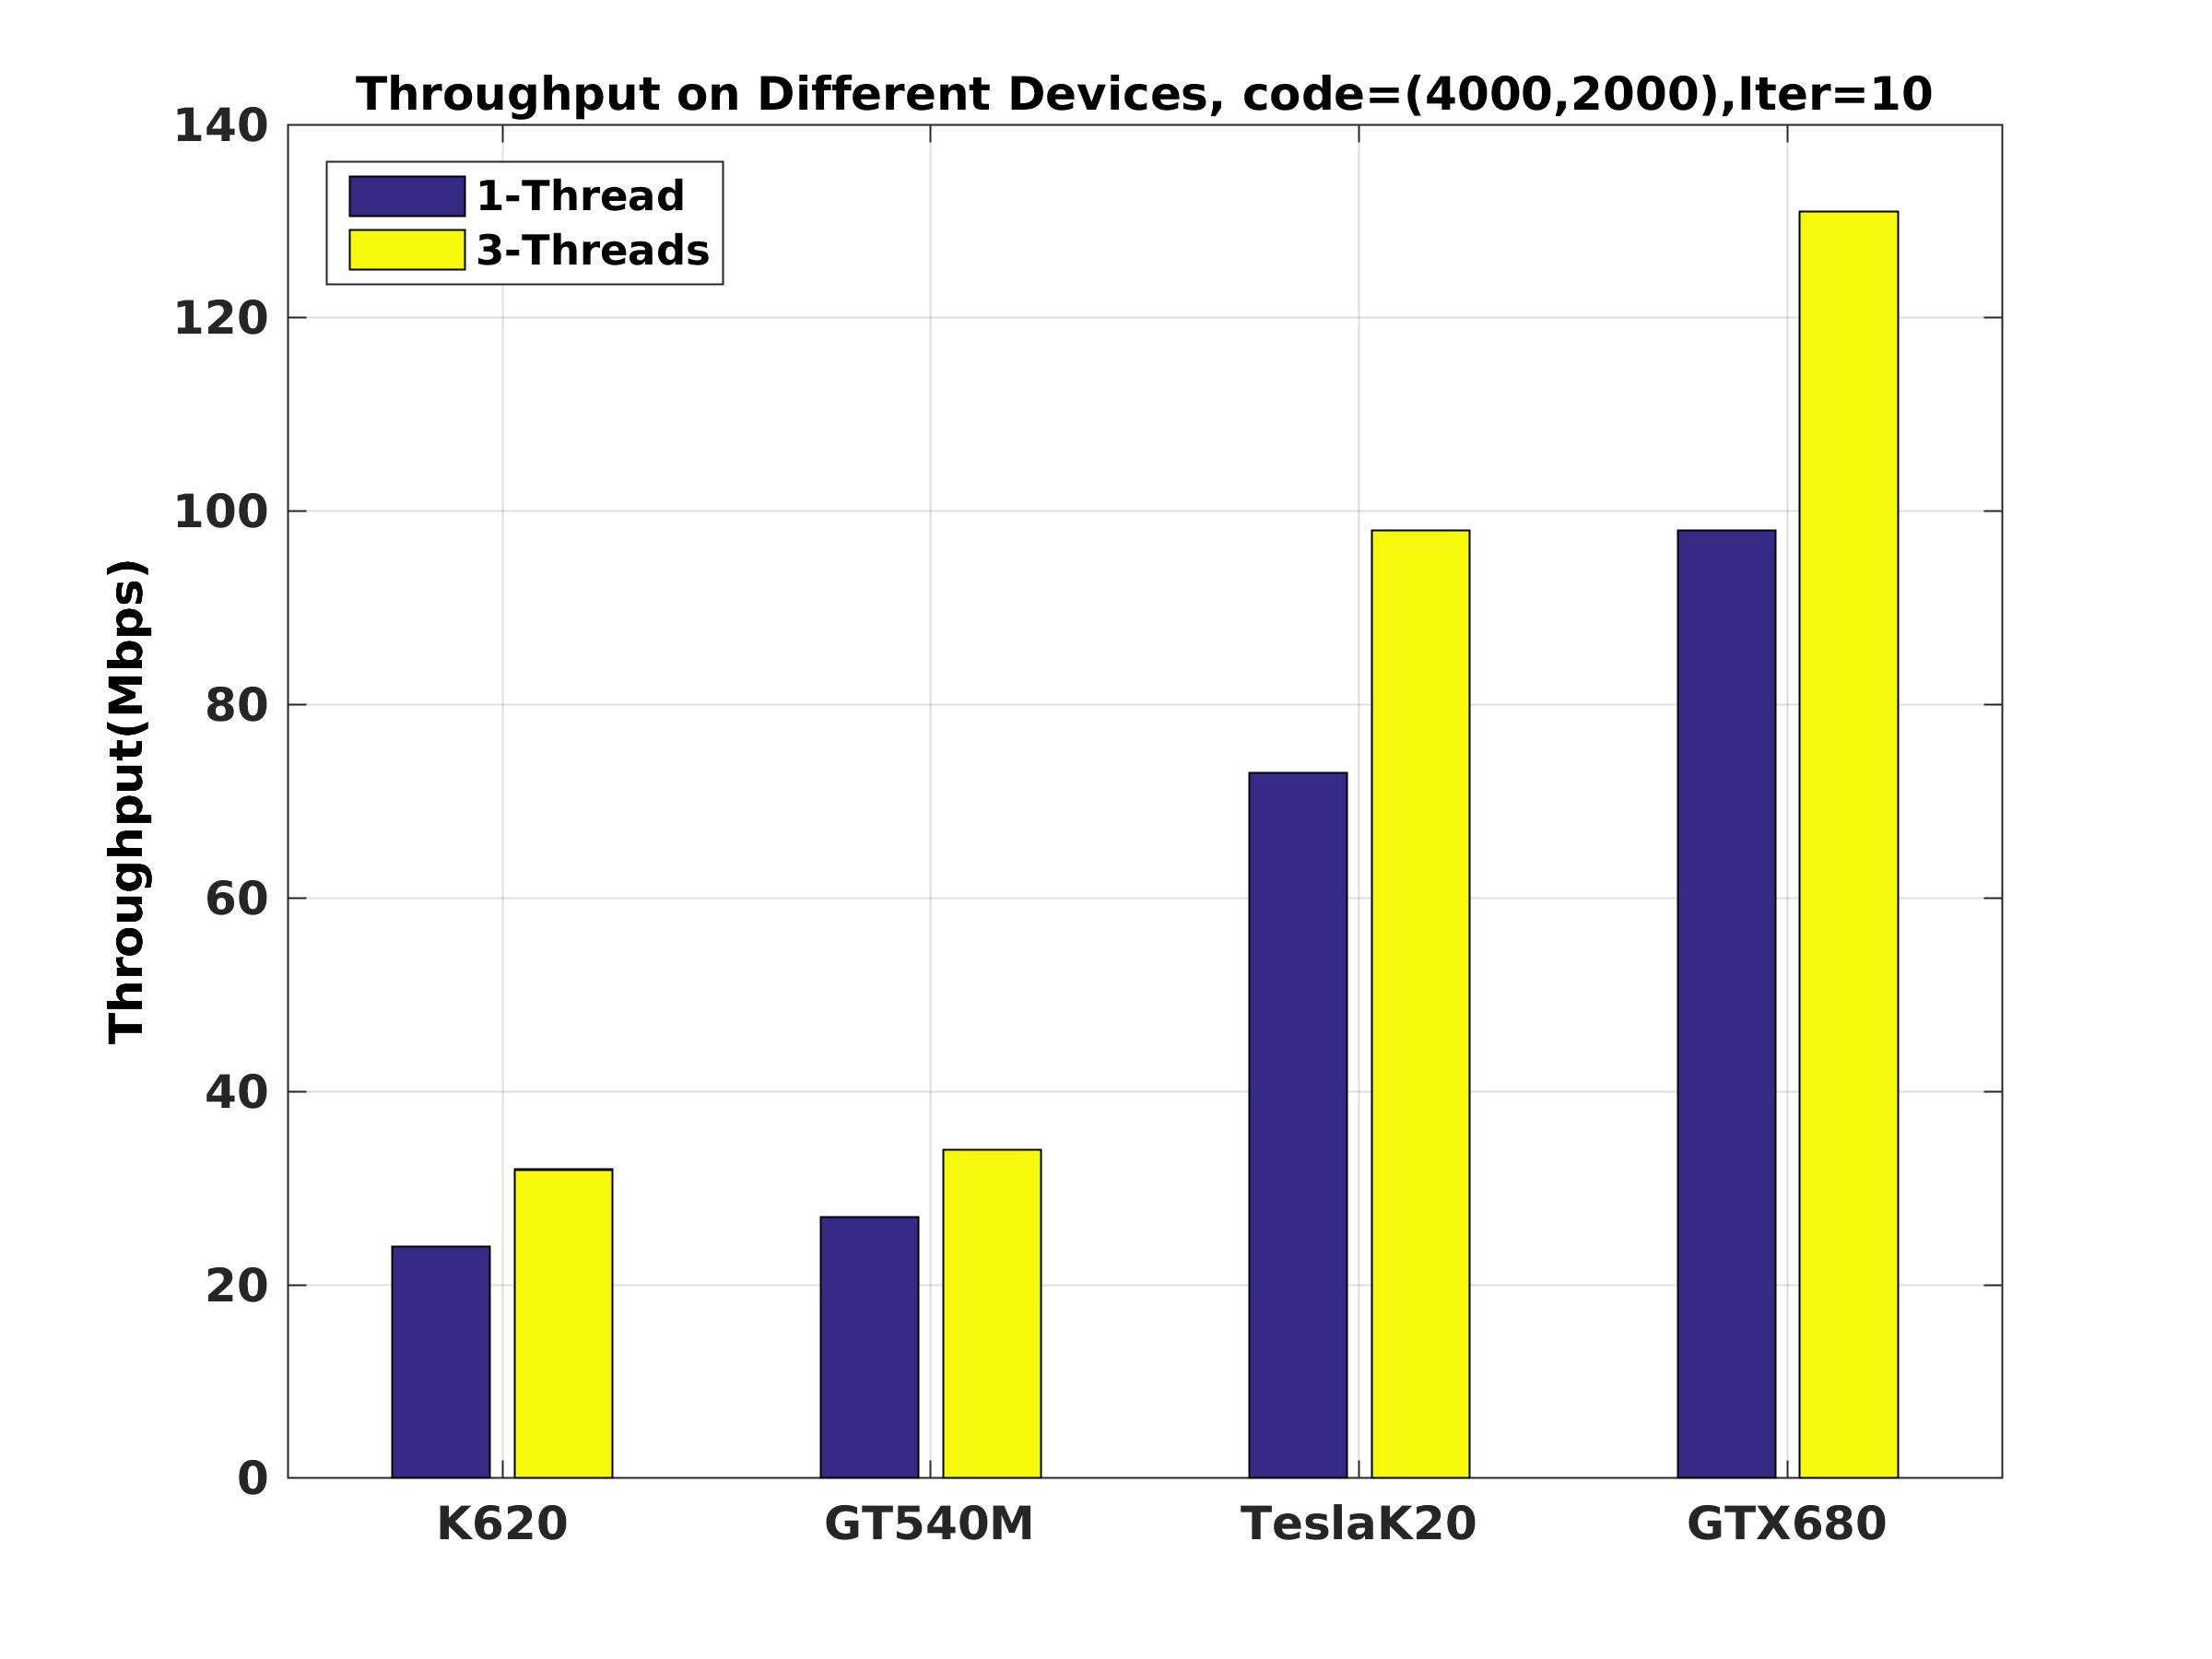
\includegraphics[width=0.65\textwidth]{img/c_4k_10.jpg}
    \caption{code=(4000,2000)}
  \end{figure}
  \end{frame}
  
\section{Conclusion}

\begin{frame}
  \frametitle{Conclusion}
  \begin{itemize}
  \item An stream-based approach for GPU-based LDPC decoding on embedded devices was introduced 
  \item Validating, Scalability Results were shown
  \end{itemize}

\end{frame}

\begin{frame}
  \frametitle{Thank You}
  \begin{figure}
    
\includegraphics[width=0.65\textwidth]{img/thank-you.jpg}
  \end{figure}

\end{frame}

\end{document}
